\section{Grundlagen zur Segeleinstellung}\label{sec:principles}
In diesem Kapitel wird grob auf die Bedeutung und Funktionsweise der Segelsteuerung eingegangen. Nachfolgende Informationen basieren auf dem Wissensstand der Vorgruppe, in deren Arbeit auf genauere Details zu dieser Thematik verwiesen wird. Eine Skizze, die daraus entnommen wurde, veranschaulicht den Sachverhalt des Segelanstellwinkels:
\begin{figure}[H]
	\centering
	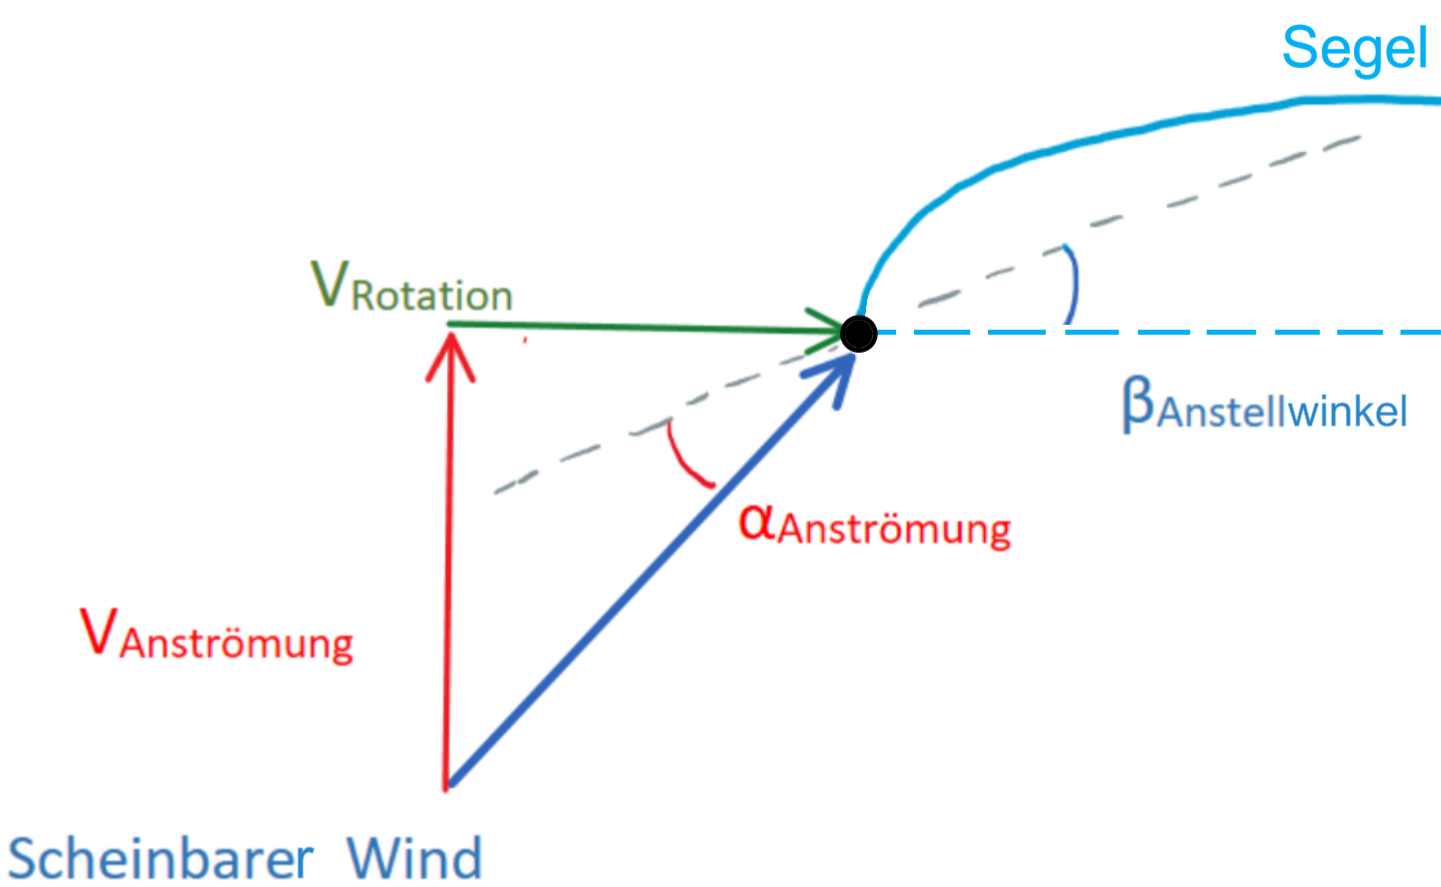
\includegraphics[width=0.6\textwidth]{images/Sailwind/sailPitchAngle.png}
	\caption{Segeltheorie: Scheinbarer Wind und Anstellwinkel}
	\label{fig:sailPitch}
\end{figure}
\noindent
Bei einem Segelboot beeinflusst der Fahrtwind den wahren Wind (hier \textit{Anströmung}) zu einem scheinbaren Wind, der effektiv in das Segel bläst. Ähnlich verhält es sich bei einem in diesem Fall segelartigen Rotorblatt, dass den Wind durch die erzeugte Rotation ablenkt. Verändert sich die Anströmungsgeschwindigkeit, muss der Anstellwinkel des Segels entsprechend angepasst werden, sodass der resultierende scheinbare Wind möglichst effizient vom Segel aufgenommen und in Rotation umgewandelt wird. So existiert zu jeder Windgeschwindigkeit ein optimaler Anstellwinkel. Diese Anpassung wird auch als Trimmen des Segels bezeichnet.\\

\noindent
Wie bereits in der Einleitung erwähnt soll bei einer Windgeschwindigkeit von 14 m/s eine Leistung von 5 kW erzeugt werden. Damit diese auch bei stärkerem Wind konstant abrufbar ist, soll die Segelfläche durch Einrollen verkleinert werden. \autoref{fig:powerCurve} zeigt die erwartete Leistungskurve in Abhängigkeit der Windstärke bei gezielter Trimmung und Rollung der Segel:
\begin{figure}[H]
	\centering
	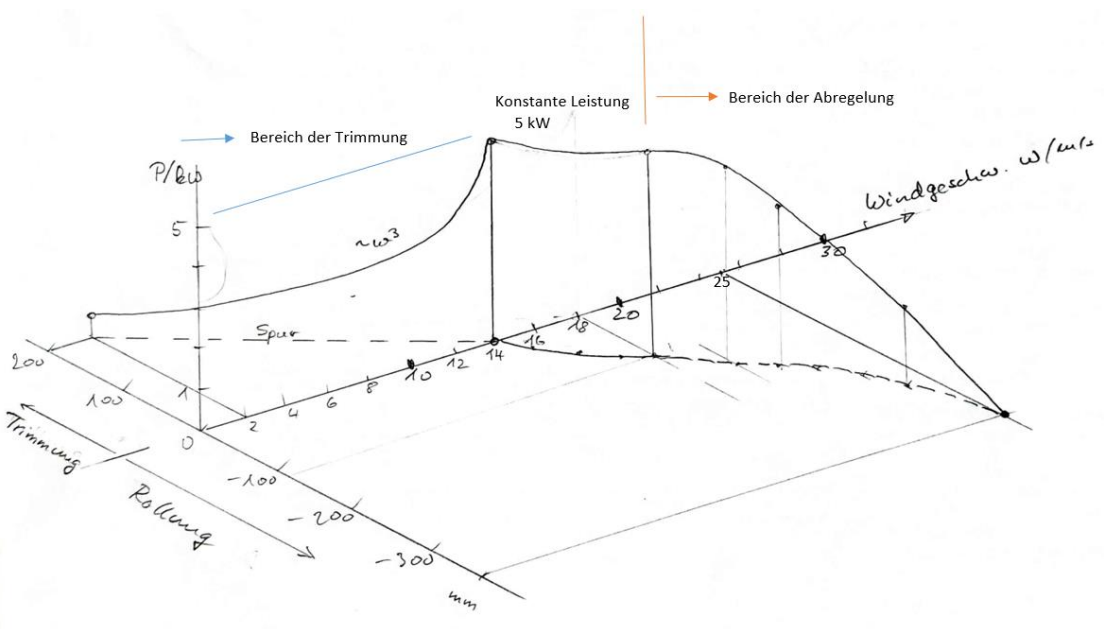
\includegraphics[width=1.0\textwidth]{images/Sailwind/powerCurve.png}
	\caption{SAILWIND Leistungskurve nach Prof. Schwechten}
	\label{fig:powerCurve}
\end{figure}
\noindent
Die Seilführung der Segel (siehe \autoref{fig:sailWindMill}) ermöglicht dabei einen fließenden Übergang zwischen Rollung und Trimmung durch eine gemeinsame Zugbewegung aller Seile parallel zur Rotorwelle, die mithilfe der Linearführung ausgeführt werden soll. Bei einer Einschaltgeschwindigkeit von 1 bis 2 m/s sollen die Segel vollständig getrimmt und ausgerollt sein. Bis zur Nenngeschwindigkeit von 14 m/s befindet sich das System im Teillastbereich, in dem der Anstellwinkel schrittweise reduziert werden soll, um stets die optimale Leistung herauszuholen. Mit weiterem Anstieg der Windgeschwindigkeit beginnt der Volllastbereich, in dem die Segel immer weiter eingerollt werden, um die Spitzenleistung von 5 kW zu erhalten. Ab einem kritischen Wert von ca. 18 m/s soll ein Abregelungsprozess durchgeführt werden.   